\documentclass[12pt, a4paper]{book}%, oneside

\usepackage[headings]{fullpage}
\usepackage{setspace}

% \usepackage[top=1.5cm,right=1.5cm,bottom=1.5cm,left=1.5cm]{geometry}
% \usepackage{fancyhdr}
% \setlength{\headheight}{20pt} 
% \usepackage{graphics}
\usepackage{graphicx}
\usepackage{float}
\usepackage{subfig}
\usepackage{array}
% \usepackage{xtab}
\usepackage{multirow}
\usepackage{booktabs}
\usepackage{appendix}
\usepackage[pdfborder={0 0 0}, colorlinks=true, linkcolor=black, citecolor=blue]{hyperref}
\usepackage[printonlyused]{acronym}
\usepackage{algorithmic}
\usepackage{algorithm}
\usepackage{ifpdf}
\usepackage{listings}
\usepackage{verbatim}
\usepackage[rgb,dvipsnames]{xcolor}
% \setlength{\parindent}{0pt}

\newcommand{\submissionDay}{XX}
\newcommand{\submissionMonth}{July}
\newcommand{\submissionYear}{20XX}
\newcommand{\submissionDate}{\submissionDay~\submissionMonth,~\submissionYear}
\newcommand{\typeOfThesis}{Bachelor Thesis}

\newcommand{\titleOfThesisOne}{The Halef Book}

\newcommand{\authorOfThesis}{Ahmed Elmalatawy}
\newcommand{\supervisorOne}{Prof. Dr. David S{\"u}ndermann}

\newcommand{\includefig}[4]{
    \begin{figure}[ht]
     \centering
      \includegraphics[width=#1\textwidth]{images/#2}
      \caption{#3}
      \label{#4}
    \end{figure}
}

\newcommand{\includefigWSC}[5]{
    \begin{figure}[ht]
     \centering
      \includegraphics[width=#1\textwidth]{images/#2}
      \caption[#3]{#4}
      \label{#5}
    \end{figure}
}

\newcommand{\includeeps}[4]{
\includefig{#1}{#2.eps}{#3}{#4}
}

\newcommand{\includeepsWSC}[5]{
\includefigWSC{#1}{#2.eps}{#3}{#4}{#5}
}


\ifpdf
\pdfinfo {
	/Author (\authorOfThesis)
	/Title (\titleOfThesisOne)
	/Subject (\typeOfThesis)
	/Keywords ()
	/CreationDate (D:20090707085533)
}
\fi

\begin{document}
% \overfullrule=5pt
\pagestyle{plain}
\pagenumbering{Roman}

\newcommand{\titlePage}{

\thispagestyle{empty}
\begin{center}

  \textbf{Fakult{\"a}t Technik}\\[1mm]
  \textbf{Studiengang Informatik}\\[1mm]
  \textbf{Duale Hochschule Baden-W{\"u}rttemberg, Stuttgart}\\[1mm]
	
\includegraphics[width=6cm]{resources/images/DHBW-logo.png}

  \vspace{0.5cm}

	\textbf{Faculty of Media Engineering and Technology}\\[1mm]
	\textbf{German University in Cairo}\\[1mm]
	
\includegraphics[width=6cm]{resources/images/GUC-logo-new.png}
	
	\vspace{2cm}
	\doublespacing
	{\Huge \textbf{\titleOfThesisOne}}\\
  {\large \textbf{An introduction to the first open-source, industry standards compliant Spoken Dialog System}}\\
	\singlespacing
	\vspace{2cm}
	{\large \textbf{\typeOfThesis}}\\
	
	\vfill
	\parbox{1cm}{
  		\begin{large}
    			\begin{tabbing}
       			Author: \hspace{2cm}  
        			\=\authorOfThesis\\[2mm]
      			Supervisor: 
        			\>\supervisorOne\\[2mm]
%				\>\supervisorTwo\\[2mm]
%				\>\supervisorThree\\[2mm]
%      			Submission Date: 
%        			\>\submissionDate\\
    			\end{tabbing}
  		\end{large}
	}\\
\end{center}
\clearpage
}
%++++++++++++++++++++++++++++++++++++++++++++++++++++++++++++++++++++
\titlePage
%\thispagestyle{empty}\ \clearpage
%\titlePage
%++++++++++++++++++++++++++++++++++++++++++++++++++++++++++++++++++++
%\thispagestyle{empty}
%This is to certify that:
%\begin{itemize}
%\item[(i)] the thesis comprises only my original work toward the Bachelor Degree
%\item[(ii)] due acknowlegement has been made in the text to all other material used
%\end{itemize}

%\vspace{2cm}
%\begin{flushright}
%\rule[0mm]{6cm}{0.2mm}\\
%\authorOfThesis\\
%\submissionDay~\submissionMonth,~\submissionYear\\
%\end{flushright}
%\clearpage


%\chapter*{Acknowledgments}
\addcontentsline{toc}{chapter}{Acknowledgments}
\label{chap:ack}
\begin{center}
  \begin{large}
    \textit{ \normalsize
    To my family: Azza and Laila\\
  Thank you for your infinite support}
  \end{large}
\end{center}


\chapter*{Abstract}
% \addcontentsline{toc}{chapter}{Abstract}
\label{chap:abstract}
Spoken Dialog Systems and virtual voice assistants are of increasing importance in today's tech scene.
Virtual voice assistants are constantly increasing the accessibility and efficiency of using technology and so, no smart phone ships without one now.
Companies such as Google and Apple have taken specific interest in this field as they aim to develop more accurate and domain free virtual voice assistants.
In the DHBW Spoken Dialog Systems Research Lab, Halef, a new \ac{sds} was developed.
It consists of three main parts; Asterisk, Cairo and \ac{jvxml}.
Those three parts are installed on different servers forming a distributed architecture, with the servers communicating using the industry standards compliant protocols; \ac{sip} and MRCP.
This work describes how Halef functions, with its different components and distributed architecture, as well as the several changes that were made to each component to suit Halef's needs, improving its efficiency and widening its capabilities. 


\tableofcontents
  % \addcontentsline{toc}{chapter}{Contents}
\clearpage 

\pagestyle{headings}
\pagenumbering{arabic}

% \setlength\parskip{15pt}
%\setlength\parskip{.5\baselineskip plus .2\baselineskip
%	minus .4\baselineskip}
% \setlength\parskip{.5\baselineskip \@plus .1\baselineskip \@minus ..1\baselineskip}


\chapter{Introduction}
\label{chap:intro}

Over the past few years, conversational agents have grown in importance, conquering the world of technology by finally being available even in the smallest of devices that everyone has nowadays, smartphones.
Conversational agents have been widely used for years in a variety of applications even before smartphones came by, like phone call routing and other simple, limited domain applications.
But in the smartphones age, all of today's smartphones ship with a virtual voice assistant as big tech companies such as Google, Microsoft and Apple compete in providing the most functionality through such assistants, enabling their users to control their phones hands-free.
However, most of these advancements are proprietary software and the open source community is yet to catch up.

This work describes Halef, an open source, industry standards compliant spoken dialog system, which aims at bridging that gap between proprietary software and it's open source counterpart.
Halef works in a unique distributed architecture, splitting it into three main components, with the ability to split those three main components even further giving a high degree of flexibility and easily allowing multiple different architectures to suit each use case.
In addition to all that, all protocols that Halef runs on; SIP and MRCP/RTP, are industry standards compliant, making it suitable and trusted for use in industry as well as research.
The Halef application development language, JVXML, is also widely recognized in the community and many proprietary softwares out there already use it as well to define their applications.
So, with all that in mind, we will jump into the nitty gritty details of Halef in the next few sections, describing how it works as well as how to tweak it for use in different areas of application with a variety of distributed architectures.

\section{Objectives} \label{sec:s1}
The main goal of this work is to describe Halef in as much detail as possible, from the conceptual and architectural level, to the classes distribution and actual code level.
With three independent servers forming the backbone of Halef, each will be described in detail as to how it runs, its own architecture and finally, how it works to serve the requests it receives to contribute to the work of the whole system.
Several practices and areas for change and improvement will be pointed out throughout the whole book and finally summarized in the final chapters.
Some applications that have been integrated and tested with Halef will also be included to demonstrate how Halef can serve different apps as well as how to overcome some difficulties with needed features that are not part of the system yet.

\section{Structure}
This book starts the walk through Halef by describing the first server, the Cairo server, in chapter \ref{chap:cairo}.
This chapter will go into Cairo's architecture and how to start its different components.
It then describes the lifecycle of the five main requests this server has to handle, the SIP invite, SIP bye, MRCP recognize, MRCP record and MRCP sythesize requests.
\par
The next chapter, \ref{chap:jvxml}, describes the JVXML server, starting from parsing the application file to communicating with the Cairo server to satisfy the regonition and synhtesis requests.
\par
Finally, some applications that have been already integrated into Halef will be described, in addition to the suggested future work on the system, before concluding the book.


\chapter{Cairo Server}\label{chap:cairo}
The Cairo server serves as the main hub for managing Halef's resources for speech recognition and synthesis.
It works as a stand-alone server waiting for any recognition or synthesis requests from the \ac{jvxml} server. It then performs the desired operations and replies to the \ac{jvxml} server with the operations' results.
The Cairo server starts three different threads; a resource server thread, a receiver resource thread and a transmitter resource thread.
The main architecture of the Cairo server is described in figure~\ref{fig:cairoserver}.
In its communication with the \ac{jvxml} server, three protocols are used; \ac{sip} for call initiation and ending, and MRCP over RTP for audio streaming using VoIP in addition to sending and receiving recognition/synthesis requests and responses.
With this distinction, two different types of request flows arise; the \ac{sip} request life cycle and the MRCP request life cycle, each of which will be described in the following sections.
But first, let's have a look at how to configure and start the Cairo server.
\begin{figure}[h]
  \centering
  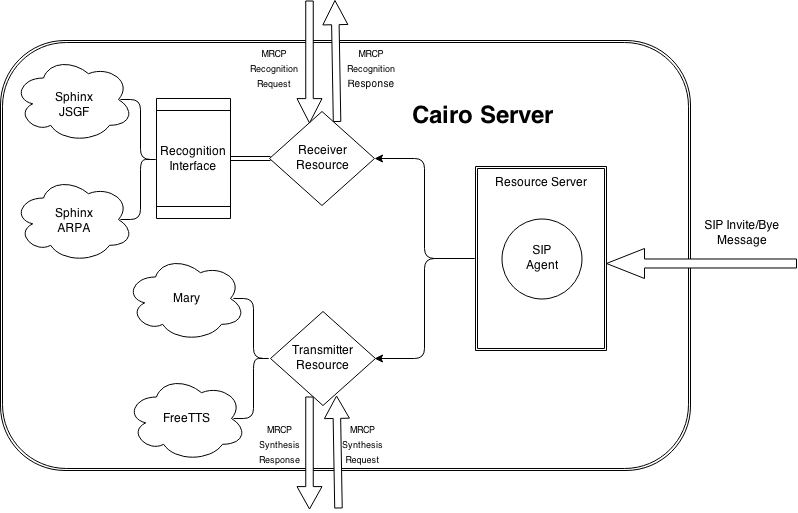
\includegraphics[width=11cm]{resources/images/Cairo-Server.png}
  \caption{Cairo Server Architecture}
  \label{fig:cairoserver}
\end{figure}

\section{Configuring the Cairo Server}
Configuring the Cairo server is fairly simple and quick, if you understand the basic, needed components.
The configuration is split into two main parts; receiver and transmitter, as you can see in listing~\ref{code:cairoconfig}.
\lstset{
  language=xml,
  tabsize=2,
  caption=Sample Cairo Config File,
  label=code:cairoconfig,
  basicstyle={\small\ttfamily},
  keywordstyle=\color{blue},
  commentstyle=\color{OliveGreen},
  stringstyle=\color{red},
  emph={cairo, resources, resource},emphstyle={\color{blue} \bf},
  numbers=left,
  numberstyle=\small,
  breaklines=true,
  aboveskip=10pt,
  belowskip=10pt
}
\lstinputlisting{resources/files/cairo-config.xml}

\subsection{Configuring the Receiver Resource}
The configuration of the receiver resource is specified in the \lstinline$<resource type="receiver">$ part of the Cairo configuration file.
This is split into a few main parts:
\begin{description}
  \item[baseGrammarDir] This is where to store the grammar file for recognition if it is sent over the network to the Cairo server. This functionality is currently disabled as only the grammar file's URL is sent over the network.
  \item[baseRecordingDir] This is where to save the speech utterances as wav files after the recording process is done by the \textit{SphinxRecorder}. 
  \item[engines] This is the maximum number of recognition engines per pool.
  \item[ipAddress] This is to specify the IP address of the resource. You generally don't need to specify this as the IP address is obtained automatically.
  \item[maxConnects] This is the maximum number of allowed parallel sessions to connect to this receiver resource.
  \item[mrcpPort] This is the MRCP port for the receiver resource. This should be the same as the MRCP transmitter port of the \ac{jvxml} server.
  \item[name] This is the identifier for the receiver being configured. The convention is to have the name as "receiver\$index".
  \item[recorderEngines] This is the maximum number of recorder engines per pool.
  \item[rtpBasePort] This is the RTP port for the receiver resource. This should be the same as the RTP transmitter port of the \ac{jvxml} server.
  \item[sphinxConfigURL] This is the path to the Sphinx recognizer configuration file. You generally don't need to specify this if the file is compiled into the "resources/config/" folder in Cairo.
  \item[sphinxRecorderConfigURL] This is the path to the Sphinx recorder configuration file. You generally don't need to specify this if the file is compiled into the "resources/config/" folder in Cairo. 
\end{description}

\subsection{Configuring the Transmitter Resource}
The configuration of the transmitter resource is specified in the \lstinline$<resource type="transmitter">$ part of the Cairo configuration file.
This is also split into a few main parts:
\begin{description}
  \item[basePromptDir] This is where to save the synthesized speech wav file after the speech synthesizer is done. 
  \item[engines] This is the maximum number of synthesis engines per pool.
  \item[ipAddress] This is to specify the IP address of the resource. You generally don't need to specify this as the IP address is obtained automatically.
  \item[maxConnects] This is the maximum number of allowed parallel sessions to connect to this transmitter resource.
  \item[mrcpPort] This is the MRCP port for the transmitter resource. This should be the same as the MRCP receiver port of the \ac{jvxml} server.
  \item[name] This is the identifier for the receiver being configured. The convention is to have the name as "transmitter\$index".
  \item[rtpBasePort] This is the RTP port for the transmitter resource. This should be the same as the RTP receiver port of the \ac{jvxml} server.
  \item[voiceName] This is the voice to be used by the FreeTTS synthesizer.
\end{description}

\section{Starting the Cairo Server}
Now, having understood all of the moving parts in the Cairo server, let's try to run it.
To start the Cairo server, all you need to do is go to the scripts directory, then run start\_cairo.sh.
This script is going to start all three components through their respective starting scripts that can be found in Cairo's bin folder.
\lstset{
  language=bash,
  tabsize=2,
  caption=Cairo Starting Script,
  label=code:startcairo,
  basicstyle={\small\ttfamily},
  emph={bash, sleep},emphstyle={\color{blue} \bf},
  numbers=left,
  numberstyle=\small,
  breaklines=true,
  aboveskip=10pt,
  belowskip=10pt
}
\lstinputlisting{resources/files/start_cairo.sh}
% more description on how Cairo starts goes here
Firstly, the resource server is started through its script \textit{rserver.sh}.
This scripts launches the server and passes some needed arguments like the SIP port to be used to communicate with the \ac{jvxml} server.
The resource server is given some time to initialize all of its components like setting up the SIP channel.
\lstset{
  language=bash,
  tabsize=2,
  caption=Cairo Resource Server Starting Script,
  label=code:startcairoresourceserver,
  basicstyle={\small\ttfamily},
  %emph={bash},emphstyle={\color{blue} \bf},
  emph={CLASS, \$CLASS},emphstyle={\color{magenta}},
  numbers=left,
  numberstyle=\small,
  breaklines=true,
  aboveskip=10pt,
  belowskip=10pt
}
\lstinputlisting{resources/files/rserver.sh}
Secondly, the receiver resource thread is launched and passed the Cairo configuration file as well as the resource name to fetch from the config file.
\lstset{
  language=bash,
  tabsize=2,
  caption=Cairo Receiver Resource Starting Script,
  label=code:startreceiver,
  basicstyle={\small\ttfamily},
  %emph={bash, sleep},emphstyle={\color{blue} \bf},
  emph={CLASS,\$CLASS,CAIRO_CONFIG,\$CAIRO_CONFIG,RES_NAME,\$RES_NAME},emphstyle={\color{magenta}},
  numbers=left,
  numberstyle=\small,
  breaklines=true,
  aboveskip=10pt,
  belowskip=10pt
}
\lstinputlisting{resources/files/receiver1.sh}
Lastly, the transmitter resource thread is started and passed the same kind of arguments as the receiver resource
\lstset{
  language=bash,
  tabsize=2,
  caption=Cairo Transmitter Resource Starting Script,
  label=code:starttransmitter,
  basicstyle={\small\ttfamily},
  emph={CLASS,\$CLASS,CAIRO_CONFIG,\$CAIRO_CONFIG,RES_NAME,\$RES_NAME},emphstyle={\color{magenta}},
  numbers=left,
  numberstyle=\small,
  breaklines=true,
  aboveskip=10pt,
  belowskip=10pt
}
\lstinputlisting{resources/files/transmitter1.sh}
Now that the Cairo server is up and running, it is ready to receive call initiation requests over \ac{sip}, so, let's have a look at the \ac{sip} requests life cycle.


%%%%%%%%%%%%%%%%%%%%%%%%%%%%%%%%%%%%%%%%%%%%%%%%%%%%%%%%%%%%%%%%%%
%%%%%%%%%%%%%%%%%%%%%%%%%%%%%%%%%%%%%%%%%%%%%%%%%%%%%%%%%%%%%%%%%%

\section{SIP Request Life Cycle}
As the calls flow into Halef, there should be a way to communicate the call initialization and termination requests between all three servers.
The \ac{sip} protocol is used for this exact purpose.
\ac{sip} provides two main types of requests, namely, an invite and a bye request, each of which is self explanatory to the nature of its purpose.
In the following subsections, we're going to look at how Cairo prepares itself for sending and receiving \ac{sip} requests, as well as, how it reacts to each type of \ac{sip} requests.

\subsection{Setting Up \ac{sip} in Cairo}
The \ac{sip} service is set up in Cairo's resource server thread as it acts as the main hub for receiving and handling the different types of \ac{sip} requests.
The resource server, represented by the \textit{org.speechforge.cairo.server.resource.ResourceServerImpl} class, implements a \ac{sip} session listener interface that allows it to work with the \ac{sip} protocol.
When the resource server thread is first run, it receives its SIP parameters from the command line launching it, configures its own SIP agent accordingly and launches it, making the Cairo server ready for listening to SIP requests.
The SIP agent is the main responsible for sending and receiving SIP requests and responses while the resource server is the one that determines how Halef uses and handles such requests.
Once the SIP agent receives an invite request, it calls the resource server's \textit{processInviteRequest} method that continues on to process and act upon such request.
Similarly, when the SIP agent receive a bye request, it calls the resource server's \textit{processByeRequest} method that processes and acts upon such request.
Both types of requests initialize a sequence of operations to be done by the Cairo server, which are described in detail in the following sections.

\subsection{\ac{sip} Invite Request}
As mentioned earlier, once the SIP agent receives an invite request, it calls the resource server's \textit{processInviteRequest} method which then initiates a series of operations through the \textit{invite} method.
The \textit{invite} method iterates through the MRCP channels that are included in the \ac{sdp} message the invite request is outlined in.
It looks for three types of channels; receiver, recorder and transmitter channels.
For each channel, its ID is extracted, formatted and included among other attributes in the media description for such channel.
This step serves to identify the resources requested by the \ac{jvxml} server for this SIP session by setting a receiver flag if a receiver or recorder channel is encountered and setting a transmitter flag if a transmitter channel is found.
Once the processing of all sessions is done, the two flags are checked and the suitable resources are requested accordingly.

\subsubsection{Requesting a Resource}
The Cairo server functions in a kind of service based approach, having its different resources running on separate threads or maybe even servers, taking advantage of Java's \ac{rmi} API to glue all the parts together.
As mentioned earlier, the Cairo server is composed of three main threads; a resource server, a receiver resource and a transmitter resource.
The SIP invite message is received on the resource server thread, but it then needs to request the different resources that are needed for the call, although they are running on other threads.
So how is this done?
The resource server is always started first as seen earlier.
As it starts, it initializes a resource registry through the \textit{org.speechforge.cairo.server.resource.ResourceRegistryImpl} class.
This resource registry serves as the connective of all three threads.
The way it operates is that the registry is hosted on a server, the resource server, then as every resource is started, it is provided the address of this registry to which it should register its resource object through Java's \ac{rmi} API.
Whenever the resource server then needs a resource of some type, it goes to this resource registry and asks to get a resource object of that type.
If a free resource of that type is found, it is given to the resource server which then binds it to the SIP session it wants to initiate by calling the resource's \textit{invite} method, supplying it with the invite request's \ac{sdp} message in addition to the SIP session's ID.

\subsubsection{Requesting a Receiver Resource}
Before getting into what happens when a receiver resource is tied to a certain \ac{sip} session, let's first see how a receiver resource is structured.
The receiver resource has three different object pools; a recognition one, a recorder one and a RTP stream replicator one.
However, the recognition one is replaced by a recognition interface that will handle all different types of recognition engines to provide flexibility.
It also has a MRCP server socket to communicate with the \ac{jvxml} server over MRCP once the channels are set up.
When the \textit{invite} method of a receiver resource is called, a series of operations is triggered to set up the MRCP channels and borrow the necessary objects from their respective object pools.
First, all of the receiver and recorder channels are extracted from the \ac{sdp} message then the suitable resources are allocated according to each channel's media descriptor.
For both types of channels, a RTP stream replicator object is borrowed from its respective pool and the MRCP channel is then registered with the MRCP server socket.
If the channel is a recognition channel, it is allocated an instance of the recognition interface to be passed to the \textit{RTPRecogChannel} along with the borrowed replicator instance.
On the other hand, if the channel is a recording one, a recorder engine is borrowed from its respective object pool then passed to the \textit{RTPRecorderChannel} along with the borrowed replicator object, the recording directory extracted from the configuration file and a content descriptor describing the media file type in which to save the recorded audio stream (Wave in our case).
The way the channel resources are mapped to the session is through the \textit{org.speechforge.cairo.server.resource.ResourceSession} class which maintains a \textit{java.util.Map} mapping the SIP session ID to the MRCP channel ID which in turn maps to the resources bound to each channel.
This setup provides access to all channels in a SIP session in addition to all the resources that the Cairo server allocated to each session even after it's done processing the SIP invite request.

\subsection{SIP Bye Request}
As mentioned earlier, once the SIP agent receives a bye request, it calls the resource server's \textit{processByeRequest} method.
This method aims at releasing all of the resources that are bound to the session being closed.
It iterates through all of the resources in that session calling the \textit{bye} method of each resource.
As we have only two types of resources, transmitter and receiver, we will examine the bye methods for both resources.

\subsubsection{Releasing a Receiver Resource}
The receiver resource has a few bound resources that should be released once the call is terminated.
The SIP session's ID is passed to the \textit{bye} method, enabling it to retrieve the session's resources from the \textit{ResourceSession} class.
It then goes through all of the resources bound to the session, signaling the MRCP server to close the opened channels and shutting down the \textit{RTPStreamReplicator}s and returning them to their pool.
It finally removes the session from the \textit{ResourceSession} map.

%%%%%%%%%%%%%%%%%%%%%%%%%%%%%%%%%%%%%%%%%%%%%%%%%%%%%%%%%%%%%%%%%%
%%%%%%%%%%%%%%%%%%%%%%%%%%%%%%%%%%%%%%%%%%%%%%%%%%%%%%%%%%%%%%%%%%

\newpage
\section{MRCP Recognition Request Life Cycle}

\begin{figure}[h]
  \centering
  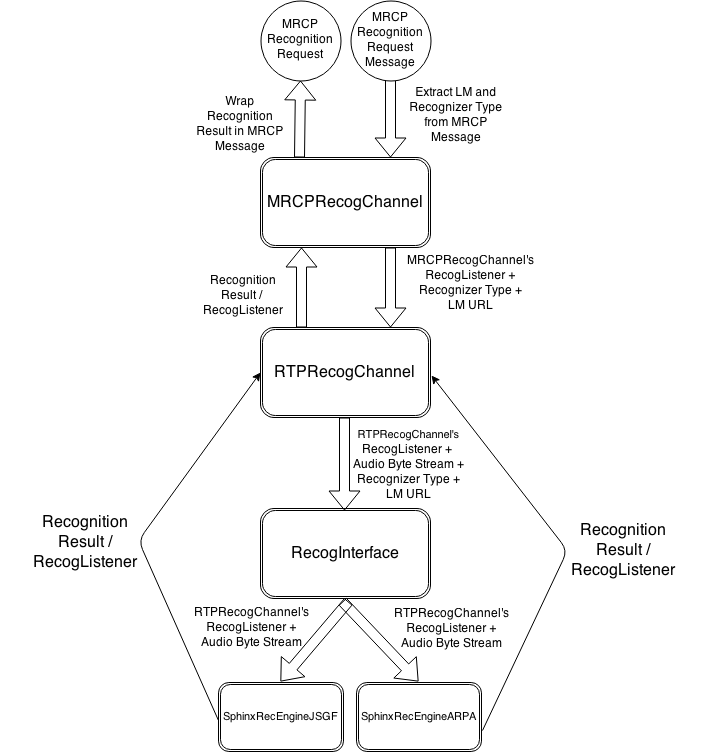
\includegraphics[width=11cm]{resources/images/MRCP-Recognition-Request-Lifecycle.png}
  \caption{MRCP Recognition Request Life Cycle}
  \label{fig:mrcprecognitionrequestlifecycle}
\end{figure}

\subsection{MRCP Message Parsing and Recognition Preparation}
\label{parsemrcp}
When the MRCP recognition channels are setup and the necessary resources allocated in the SIP invite request processing, the bound receiver resource is then ready to receive speech recognition requests over MRCP.
During the channels setup, an object of type \textit{org.speechforge.cairo.server.recog.MrcpRecogChannel} is instantiated and added to the MRCP server of the receiver resource as the manager of the recognition part for such session.
When a recognition request is sent by the \ac{jvxml} server over a certain MRCP channel, it fires the \textit{recognize} method in the respective \textit{MrcpRecogChannel}.
This method receives the MRCP message, does some preprocessing accordingly, then delegates the actual recognition part to the allocated \textit{org.speechforge.cairo.server.recog.RTPRecogChannel}.
After doing some checks on the current state of this channel and whether this message has any contents, the \textit{invite} method proceeds to parse the recognition request, extracting first the requested recognizer type.
The currently supported recognizer types are Sphinx JSGF and Sphinx ARPA recognizers specified in the message as "application/jsgf" and "application/arpa" respectively.
It then proceeds to extract the URL of the language model file to be used in satisfying this recognition request.
\lstset{
  language=java,
  tabsize=2,
  caption=Extract Application Type and Language Model's URL from MRCP Message,
  label=code:mrcprecogchannel_getgrammarurl,
  basicstyle={\small\ttfamily},
  emph={request},emphstyle={\color{magenta}},
  numbers=left,
  numberstyle=\small,
  breaklines=true,
  aboveskip=10pt,
  belowskip=10pt
}
\lstinputlisting{resources/files/mrcprecogchannel_getgrammarurl.java}
At this point, the recognition process is delegated to the \textit{RTPRecogChannel} through passing the extracted information from the MRCP message along with a callback listener to the \textit{RTPRecogChannel.recognize} method.\\
The \textit{RTPRecogChannel} handles all the dirty work involved in the recognition process, setting up data streams and needed recognizers, then calling the suitable methods through the recognition interface to complete the recognition process.
It starts by extracting the data stream from the \textit{RTPStreamReplicator} into the format that will be used in all later stages which is \textit{javax.media.protocol.PushBufferDataSource}.
It then starts the recognition process through the recognition interface, implemented through the class \textit{org.speechforge.cairo.server.recog.RecogInterface}, by first activating the needed recognizer through calling the \textit{RecogInterface.activateRecEngine} method with the specified application type and the language model's URL.
The actual recognition process is started then through the \textit{RecogInterface.startRecognition} method passing to it the previously extracted \textit{PushBufferDataSource} and a callback listener.
From this point onwards, the recognition interface will assume leadership of the process, picking the suitable recognizer that the application has asked for, starting recognition through this recognizer, then handing the result back to the \textit{RTPRecogChannel} through the callback listener.

\subsection{Recognition Interface}
In the original implementation of the Cairo server, the Sphinx recognizer was integrated within the whole system which imposed a lot of flexibility restrictions.
As the need arose for using other types of recognizers which proved to provide better results, a solution providing generality and an easy plug-in-plug-out nature had to be implemented, and this is when the recognition interface was born.
The recognition interface is basically an added layer of abstraction that separates the management of the actual recognition engines from the rest of the Cairo server.
With this addition, all the Cairo server has to do is call the generic methods provided by the recognition interface and then let it handle all the mess of managing which recognizer type to pick, which specific recognition engine to launch and how to pass the data source to this specific recognizer instance.
In addition to managing the recognition engines, the recognition interface can also implement several new functionalities like caching the recognition engines that already have a certain language model loaded in them.
Let's dive now into the details of how the recognition interface works.

\subsubsection{Managing the Different Recognition Engines}
The recognition engine needs to have a flexible way of managing the different recognition engines which assumes nothing about which recognizers are in use and which functionality they have to offer.
In order to satisfy those purposes, a \textit{java.util.HashMap} is used, mapping the unique recognizer type to recognition engines pool of that type.
This \textit{String} to \textit{ObjectPool} mapping is generic enough to represent all keys and recognizer types making adding a new recognition engine to Halef a really easy task.
When a recognition request is placed, the recognition interface will go and fetch the required engine from the relative \textit{ObjectPool} fetched from the map.

\lstset{
  language=java,
  tabsize=2,
  caption=Recognition Interface Application Type to \textit{ObjectPool} Map,
  label=code:recoginterface_map,
  basicstyle={\small\ttfamily},
  emph={_recPools},emphstyle={\color{magenta}},
  numbers=left,
  numberstyle=\small,
  breaklines=true,
  aboveskip=10pt,
  belowskip=10pt
}
\lstinputlisting{resources/files/recoginterface_map.java}

\subsubsection{Initializing the Recognition Interface}
The initialization process is pretty straight forward, creating new \textit{ObjectPool}s for the predefined recognizer types.
During the current setup, the predefined types are hard coded into the recognition interface with the application type being explicitly specified as \textit{application/jsgf} and \textit{application/arpa}.
Going forwards, such predefinition can be changed from hard coding certain types to fetching them from a certain section in the Cairo configuration file, providing more flexibility and saving on memory especially as the number of different recognizers to use becomes bigger.
However, if the recognition pool for a certain application type isn't created during the initialization phase, all is not lost.
If a certain mapping from application type to a certain object pool is specified in the Cairo configuration file, this pool can then be automatically added to the map and the recognition can start with this new type.
This feature as well is not yet implemented, but it can easily be added in the future, and the way the recognition interface is implemented fully supports that.
\lstset{
  language=java,
  tabsize=2,
  caption=Recognition Interface Initialization,
  label=code:recoginterface_initialize,
  basicstyle={\small\ttfamily},
  emph={_recPools,_config},emphstyle={\color{magenta}},
  numbers=left,
  numberstyle=\small,
  breaklines=true,
  aboveskip=10pt,
  belowskip=10pt
}
\lstinputlisting{resources/files/recoginterface_initialize.java}

\subsubsection{Activating a certain Recognition Engine and Starting Recognition}
When a recognition request is placed by the JVXML server and it reaches the recognition interface as part of the request's life cycle, the recognition interface performs the task of fetching the suitable recognition engine, loading the language model into it, then starting the recognition thread.
First of all, the \textit{RecognitionInterface.activateRecEngine} method is called, providing it with the application type and the location of the language model.
This method fetches the correct recognition pool, using the application type as the key, from the interface's map.
It then requests an available recognition engine instance from that pool to carry out this recognition request.
It is now assumed, as forced by Halef's current capabilities, that only a single recognition request will be taking place at a certain time instance and so, the resources management here is done by saving the currently requested recognition engine as well as its pool into a single instance of \textit{org.speechforge.cairo.server.recog.ActiveRecognizer}.
\lstset{
  language=java,
  tabsize=2,
  caption=Recognition Interface Recognizer Handling,
  label=code:recoginterface_recognizer,
  basicstyle={\small\ttfamily},
  emph={_activeRecog,_recPools},emphstyle={\color{magenta}},
  numbers=left,
  numberstyle=\small,
  breaklines=true,
  aboveskip=10pt,
  belowskip=10pt
}
\lstinputlisting{resources/files/recoginterface_recognizer.java}
The \textit{ActiveRecognizer} class handles the specifics of managing the current recognition engine according to its type, explicitly loading the language model in it, starting its recognition thread and finally deallocating its language model and returning it to its respective object pool once the recognition is finalized.
From that point till the end of the recognition request cycle, any functionality called to the recognition interface will be passed to the active recognizer to explicitly call the methods to perform such functionality.
With the current implementation, the \textit{ActiveRecognizer} assumes knowing the details of the recognizer types that Halef supports and hard codes test cases for each type to work with it differently.
However, for actual generality purposes, it would be better to have an interface that specifies how a recognition engine should act in general, then have every recognition engine type implement it.
This then would be the way of handling how the \textit{ActiveRecognizer} deals with the required recognition functionality, reaching a fully generic implementation that assumes nothing about the recognizer type.
\lstset{
  language=java,
  tabsize=2,
  caption=Active Recognizer Class,
  label=code:activerecognizer,
  basicstyle={\small\ttfamily},
  emph={_recEngine,_recPool,_appType},emphstyle={\color{magenta}},
  numbers=left,
  numberstyle=\small,
  breaklines=true,
  aboveskip=10pt,
  belowskip=10pt
}
\lstinputlisting{resources/files/activerecognizer.java}

Once the recognition engine is loaded into the \textit{ActiveRecognizer} instance, it can be used to initiate the recognition process through the \textit{startRecognition} method.
The results are not returned directly by this method, instead, they are returned through the recognition listeners that are passed from the \textit{MRCPRecogChannel} to the \textit{RTPRecogChannel} and then to the recognition engine through the interface.
The result is then passed up from each listener to the layer above it, till it finally reaches the \textit{MRCPRecogChannel} which then encapsulates it in a MRCP message and sends it to the JVXML server.

\subsection{Sphinx Recognition Engine}
In this section, a speech recognizer's, namely Sphinx4,  support package will be described, also giving an insight on how to integrate any speech recognizer into Halef.
Sphinx4 has the advantage of being written in Java and thus, it's easy to use its API to integrate it into Halef whose main development language is also Java.
For other recognizers that aren't written in Java, a Java API has to be provided in order to be able to integrate it into Halef, for example using SWIG for recognizers implemented in C/C++, or by providing recognition as a service.
The latter however, may need some smart design to create a Java API that simulates an integrated recognition engine to Halef while communicating with the recognition service to obtain the recognition results.
Any recognizer to be added to Halef has to have certain properties, the first is being a poolable object and the second is implementing the \textit{SpeechEventListener} interface.
The first property guarantees that we can create a pool of several recognition engine objects of that particular recognizer through its factory class, implementing the factory design pattern.
The second property is one that gives us a way to handle the different speech signals and also propagate the results to the higher levels of abstraction, namely the \textit{RTPRecogChannel} and subsequently the \textit{MRCPRecogChannel}.

\subsubsection{Speech Data Handling}
The speech data stream is passed to the recognizer through the \textit{startRecognition} method in the form of a \textit{javax.media.protocol.PushBufferDataSource}.
This stream is passed as is from the \textit{RTPRecogChannel} and should be accommodated to fit the needs of the recognizer in use.
In the case of Sphinx4, this \textit{PushBufferDataSource} is transformed into a \textit{org.speechforge.cairo.rtp.server.sphinx.RawAudioProcessor} in the \textit{startRecognition} method through the \textit{RawAudioTransferHandler} class.
The \textit{RawAudioProcessor} class is then responsible for taking the speech data's byte stream and passing it to the Sphinx4 front end to do the actual recognition.
\lstset{
  language=java,
  tabsize=2,
  caption=\textit{startRecognition} method,
  label=code:startrecognition,
  basicstyle={\small\ttfamily},
  emph={_rawAudioTransferHandler,_rawAudioProcessor,_recogListener},emphstyle={\color{magenta}},
  numbers=left,
  numberstyle=\small,
  breaklines=true,
  aboveskip=10pt,
  belowskip=10pt
}
\lstinputlisting{resources/files/startrecognition.java}

\subsubsection{Speech Event Listeners}
As the speech signal is passed as a continuous one over the RTP channel, the Sphinx front-end needs a way to figure out when the actual speech utterance, not emptiness or noise, to be recognized starts and ends.
This is done through an instance of the \textit{org.speechforge.cairo.rtp.server.sphinx.SpeechDataMonitor} class.
This object's configuration is loaded from the Sphinx configuration file, started in the recognition engine's constructor and passed to it is the recognition engine instance as the \textit{SpeechEventListener}.
When a speech start signal is encountered, the \textit{SpeechDataMonitor} broadcasts a speech start signal to all of its associated \textit{SpeechDataListeners} through the \textit{broadcastSpeechStartSignal()} method. 
Similarly, when a speech end signal is encountered, the \textit{broadcastSpeechEndSignal()} method is used to send a speech end signal to all listeners.
In the \textit{speechStarted()} method, the abstract class \textit{SphinxRecEngine} does a very simple function which is setting the call back listener to the \textit{RTPRecogChannel}'s \textit{RecogListener} passed to the recognition engine earlier through the \textit{startRecognition()} method.
At this point, we have an abstract \textit{SphinxRecEngine} class, implementing all the common behaviors of any Sphinx recognition engine disregarding its type.
We have two different types of recognition engines built over this abstract \textit{SphinxRecEngine} class, one for recognition using JSGF grammars, namely \textit{SphinxRecEngineJSGF}, and another for recognition using ARPA n-gram language models, namely \textit{SphinxRecEngineArpa}.

\subsubsection{SphinxJSGF Recognition}
The \textit{SphinxRecEngineJSGF} class is a child of the \textit{SphinxRecEngine} class, implementing the functionality of the Sphinx recognizer for JSGF grammars.
The class has an instance of \textit{edu.cmu.sphinx.jsapi.JSGFGrammar} which acts as the grammar to plug in and out of the recognizer for each different recognition request.
Before each recognition request is fulfilled, the grammar specified in the MRCP message, described before in section \ref{parsemrcp}, has to be loaded through the \textit{load(GrammarLocation)} method.
This method takes a \textit{GrammarLocation} object as a parameter and loads the specified grammar into the \textit{JSGFGrammar} object.
\lstset{
  language=java,
  tabsize=2,
  caption=\textit{load()} JSGF method,
  label=code:loadjsgf,
  basicstyle={\small\ttfamily},
  emph={_jsgfGrammar},emphstyle={\color{magenta}},
  numbers=left,
  numberstyle=\small,
  breaklines=true,
  aboveskip=10pt,
  belowskip=10pt
}
\lstinputlisting{resources/files/loadjsgf.java}

Once the grammar is loaded, the recognizer is ready to do the actual recognition through the \textit{startRecognitionThread} method.
This method will dispatch a separate thread that will initiate and follow up with the recognition process.
The \textit{run} method first starts by calling the \textit{waitForResult} method that will ask the recognition engine to do the recognition then get the recognition result.
\lstset{
  language=java,
  tabsize=2,
  caption=\textit{run()} JSGF method,
  label=code:runjsgf,
  basicstyle={\small\ttfamily},
  emph={_recogListener},emphstyle={\color{magenta}},
  numbers=left,
  numberstyle=\small,
  breaklines=true,
  aboveskip=10pt,
  belowskip=10pt
}
\lstinputlisting{resources/files/runjsgf.java}

The \textit{waitForResult} method gives the command to do the recognition through calling the \textit{recognize} method of the \textit{edu.cmu.sphinx.recognizer.Recognizer} instance that this \textit{SphinxRecEngine} has.
There are two modes for obtaining the final result, if the \textit{hotword} flag is set, then it keeps asking for recognition results until it reaches a grammatical result, otherwise, only one result is obtained and returned disregarding its grammaticality.
\lstset{
  language=java,
  tabsize=2,
  caption=\textit{waitForResult()} JSGF method,
  label=code:waitforresultjsgf,
  basicstyle={\small\ttfamily},
  emph={_jsgfGrammar, _recognizer},emphstyle={\color{magenta}},
  numbers=left,
  numberstyle=\small,
  breaklines=true,
  aboveskip=10pt,
  belowskip=10pt
}
\lstinputlisting{resources/files/waitforresultjsgf.java}

After the recognition result is obtained, it is passed upwards to the \textit{RTPRecogChannel} through the provided \textit{RecogListener} that was passed downwards during the recognition initiation phase by calling the \textit{recognitionComplete} method.

\subsubsection{SphinxARPA Recognition}
The \textit{SphinxRecEngineARPA} class is a child of the \textit{SphinxRecEngine} class, implementing the functionality of the Sphinx recognizer for ARPA statistic language models.
The class has an instance of \textit{edu.cmu.sphinx.linguist.language.ngram.SimpleNGramModel} which acts as the ARPA n-gram model to plug in and out of the recognizer for each different recognition request.
Before each recognition request is fulfilled, the language model specified in the MRCP message, described before in section \ref{parsemrcp}, has to be loaded through the \textit{load(GrammarLocation)} method.
This method takes a \textit{GrammarLocation} object as a parameter and loads the specified language model into the \textit{SimpleNGramModel} object.
\lstset{
  language=java,
  tabsize=2,
  caption=\textit{load()} ARPA method,
  label=code:loadarpa,
  basicstyle={\small\ttfamily},
  emph={_nGramModel, _linguist, _ps},emphstyle={\color{magenta}},
  numbers=left,
  numberstyle=\small,
  breaklines=true,
  aboveskip=10pt,
  belowskip=10pt
}
\lstinputlisting{resources/files/loadarpa.java}

Once the n-gram language model is loaded, the recognizer is ready to do the actual recognition through the \textit{startRecognitionThread} method.
This method will dispatch a separate thread that will initiate and follow up with the recognition process.
The \textit{run} method first starts by calling the \textit{waitForResult} method that will ask the recognition engine to do the recognition then get the recognition result.
\lstset{
  language=java,
  tabsize=2,
  caption=\textit{run()} ARPA method,
  label=code:runarpa,
  basicstyle={\small\ttfamily},
  emph={_recogListener},emphstyle={\color{magenta}},
  numbers=left,
  numberstyle=\small,
  breaklines=true,
  aboveskip=10pt,
  belowskip=10pt
}
\lstinputlisting{resources/files/runarpa.java}

The \textit{waitForResult} method gives the command to do the recognition through calling the \textit{recognize} method of the \textit{edu.cmu.sphinx.recognizer.Recognizer} instance that this \textit{SphinxRecEngine} has.
\lstset{
  language=java,
  tabsize=2,
  caption=\textit{waitForResult()} ARPA method,
  label=code:waitforresultarpa,
  basicstyle={\small\ttfamily},
  emph={_recognizer},emphstyle={\color{magenta}},
  numbers=left,
  numberstyle=\small,
  breaklines=true,
  aboveskip=10pt,
  belowskip=10pt
}
\lstinputlisting{resources/files/waitforresultarpa.java}

After the recognition result is obtained, it is passed upwards to the \textit{RTPRecogChannel} through the provided \textit{RecogListener} that was passed downwards during the recognition initiation phase by calling the \textit{recognitionComplete} method.

\chapter{JVoiceXML Server}\label{chap:jvxml}
  JVXML

\chapter{Applications}
\label{chap:applications}
In this chapter, several applications that have been already integrated into Halef will be discussed.

\section{Voice Enabled Question Answering using OpenEphyra}
This was the first application that has been built for Halef's demoing purposes.
The application's idea is to integrate OpenEphyra, a question answering system inspired by IBM's Watson, into Halef, thus creating a voice enabled service for question answering.
Of course this application had one major challenge, being how to train a generic enough language model to enable the recognizer to effectively recognize questions that have no specific domain.
For our demo, we created a small grammar consisting of a few questions and then the user calls in, asks a question out of those, the recognition result is then passed to OpenEphyra to get a suitable answer, then the answer is synthesized and played out to the user.

\section{Stuttgart's VVS Transportation System}
The second application is one that serves the city of Stuttgart, Germany through providing a service to get the next available Verkehrsverbund Stuttgart (VVS) transportation route from one station to another.
The user calls in and is asked to provide the name of the route's start station, then is prompted to provide the name of the end station and finally, the route is queried through the VVS API to get the next available route which is then prompted out to the user.
The user is prompted the number of the transportation line to take, the timing it leaves from the start station and the timing it arrives at the end station.
If the route isn't a direct one, the user is prompted the details of each and every connection in the format explained previously.
The API is queried through HTTP GET requests, and it then provides the results in XML form which then needs to be parsed to extract the details of the route, then put it in a suitable format to be passed as voice output to the user.
Since the applications for Halef are written in JVXML, the functionality to deal with the API needed to be written in another language, then the JVXML server will deal with it as a service to query and get the results.
The service to deal with the VVS API was made in Java and it actively listens to requests sent to it by the JVXML server as they communicate through JSON objects.


\chapter{Conclusion}\label{chap:concl}

In the end, here is a wrap up of what Halef is, and how it operates.
Halef, the open source, industry standards compliant spoken dialog system, consists of three main servers, namely, the Asterisk call management server, the Cairo server for recognizing, recoding and synthesizing speech and the JVXML server for parsing the applications and issuing the recognition, recoding and synthesis requests to the Cairo server.
The user call starts at the Asterisk server, which receives the user call over SIP or PSTN, then routes the user to the correct application according to the entered extension.
This call is then connected to the suitable JVXML server which will fetch the correct application file, parse it and execute it.
During the application's execution, the required recognition and synthesis requests are then sent over to the Cairo server to carry them out and return their respective results.
Speech data is passed between the servers using MRCP over RTP which follows the industry's standards and the applications are developed using JVXML, which is also widely used in speech applications, also following industry standards.


\chapter{Ongoing and Future Work}
\label{chap:todo}
As the development is ongoing in Halef, several new features are being added and a bunch of others are being improved.

\section{Areas of improvement}
Throughout the book, a few points have been pointed out as possible areas of addition or improvement.
In this section, those points will be summarized.

\subsection{Plug in - Plug out Nature for Speech Recognizers and Synthesizers}
The Cairo server was developed as a separate project and it shipped with Sphinx4 and FreeTTS integrated into it.
This integration goes into the heart of the Cairo server that it makes the job of adding other speech recognizers and synthesizers more difficult than it should be.
Ideally, Halef should provide an easy interface that allows to plug in and plug out any speech recognizer or synthesizer easily.
This would give Halef maximum flexibility and would allow it to cope with the new technologies as they roll out.
The recognition interface described earlier took a step forwards in this direction, achieving some sort of flexibility and allowing the use of two recognizer types instead of one by adding Sphinx4 ARPA to the originally present Sphinx4 JSGF recongizer.
However, the job of adding a totally different recognizer other than Sphinx4 is still an ongoing work as will be explained later.
During this process, it is expected to meet more areas where the architecture of the Cairo server will have to be changed to provide more separability between it and the Sphinx4 recognizer.

\subsection{Multiple Recognition Threads}

\subsection{Supporting more VXML tags in JVXML}

\section{New Areas of Development}

\subsection{Integrating the Kaldi Recognizer}

\appendix
\renewcommand{\appendixtocname}{Appendix}
\renewcommand{\appendixpagename}{\appendixtocname}
\addappheadtotoc
\setboolean{@twoside}{false}
\appendixpage

\chapter{Lists}
\addcontentsline{toc}{section}{List of Abbreviations}
\begin{acronym}[\hspace{3cm}]
  \acro{ac}[AC]{Acronym Without Citation}
  \acro{ac2}[AC2]{Acronym With Citation \cite{citeKey2}}
  \acro{sds}[SDS]{Spoken Dialog System}
  \acro{jvxml}[JVXML]{JVoiceXML}
  \acro{sdp}[SDP]{Session Description Protocol}
  \acro{sip}[SIP]{Session Initialization Protocol}
  \acro{rmi}[RMI]{Remote Method Invocation}
\end{acronym}
\clearpage
\listoffigures
\addcontentsline{toc}{section}{List of Figures}
\lstlistoflistings
\addcontentsline{toc}{section}{List of Listings}
%\begin{lstlisting}[label=code:cairoconfig]
%\end{lstlisting}
% \listoftables
% \addcontentsline{toc}{section}{List of Tables}


\bibliographystyle{plain}
\bibliography{bachelor}
\addcontentsline{toc}{chapter}{References}

\end{document}
